\hypertarget{particle-filters}{%
\section{Particle Filters}\label{particle-filters}}

Note

Lots to add for this section.

Particle filters are a form of sequential Monte Carlo methods used to
address the hidden Markov chain and nonlinear filtering problems.
Normally known as a non-parametric filter and separated from Kalman
Filters, we will treat them together as forms of dynamic state
estimation. It is essentially a form of a genetic algorithm applied to
state estimation and is a popular form of non-parametric alternative to
the Gaussian filters (Kalman Filter). Particle filters use a finite
number of discrete variables to approximate the posterior. The basic
algorithm for one step of the filter is given
Algorithm~\href{..\%20topic::\%20\%20Particle\%20Filter.\%20:cite:\%60thrun2005probabilistic\%60}{alg:particlefilter}.
We will use the notation that \(x_k\) is a particle, \(X_k\) is the set
of paticles, \(u_k\) is the control input and \(z_k\) is the observation
at time step \(k\).

\begin{quote}
\textbf{Input} \(X_{k-1}\), \(u_k\), \(z_k\)\\
\textbf{Output} \(X_k\)\\
Initialize \(Y\), \(X_k\) to zero.\\
\textbf{for} \(m=1\) to \(M\) \textbf{do}\\
\hspace*{0.333em}\hspace*{0.333em}Sample \(x_k^m\) from
\(p(x_k | u_k, x_{k-1}^m)\)\\
\hspace*{0.333em}\hspace*{0.333em}\(w_k^m = p(z_k|x_k^m)\)\\
\hspace*{0.333em}\hspace*{0.333em}\(Y = Y + [x_k^m]\)\\
\textbf{end for}\\
\textbf{for} \(m=1\) to \(M\) \textbf{do}\\
\hspace*{0.333em}\hspace*{0.333em}Select \(x_k^i\) from \(Y\) with
probability \(w^i_k\)\\
\hspace*{0.333em}\hspace*{0.333em}\(X_k = X_k + [x_k^i]\)\\
\textbf{endfor}
\end{quote}

The standard algorithm for resampling selects the particle based on some
probability which is proportional to the probability of the observation
given the particle, often called the weight of the particle, \(w_k\).
One approach to this is in algorithm
\href{..\%20topic::\%20\%20Resample\%20algorithm.\%20\%20Uses\%20the\%20particle\%20weights\%20to\%20set\%20the\%20sampling\%20probability.}{alg:probsample}.
In the Evolutionary Computation literature this is a form of Roulette
selection. A low variance resample approach which numerically faster can
be found in algorithm
\href{..\%20topic::\%20\%20Low\%20variance\%20resample\%20algorithm.\%20\%20This\%20algorithm\%20runs\%20faster\%20than\%20the\%20previous\%20resample\%20approach.}{alg:lowvariancesample}.
To obtain good state estimates, it may be necessary to use many
particles which can require significant computation. This is the
tradeoff when compared to Gaussian filters (Kalman Filter).

\begin{quote}
\textbf{Input} \(Y\) (particle set), \(w^i\), \(w = \sum w^i\)\\
\textbf{Output} \(X\) (resampled particle set)\\
Initialize \(X\) to zero\\
\textbf{for} \(m=1\) to \(M\) \textbf{do}\\
\hspace*{0.333em}\hspace*{0.333em}Generate \(r\), random number from
uniform distribution \((0,w)\)\\
\hspace*{0.333em}\hspace*{0.333em}\(s = 0\), \(i = 0\)\\
\hspace*{0.333em}\hspace*{0.333em}*\emph{while}* \(s < r\) \textbf{do}\\
\hspace*{0.333em}\hspace*{0.333em}\hspace*{0.333em}\hspace*{0.333em}\(s = s + w^i\)\\
\hspace*{0.333em}\hspace*{0.333em}\hspace*{0.333em}\hspace*{0.333em}\(i = i+1\)\\
\hspace*{0.333em}\hspace*{0.333em}*\emph{end while}*\\
\hspace*{0.333em}\hspace*{0.333em}\(X = X + \{x_i\}\)\\
\textbf{end for}
\end{quote}

\begin{verbatim}
k = 1
while (k<N):
    j=0
    ws = 0
    while (j < M):
        q = np.random.normal(mu1,sigma1,3)
        pftemp[j,0] = pf[j,k-1,0] + dd*(w1[k]+w2[k])*cos(x[k-1,2]) + q[0]
        pftemp[j,1] = pf[j,k-1,1] + dd*(w1[k]+w2[k])*sin(x[k-1,2]) + q[1]
        pftemp[j,2] = pf[j,k-1,2] + dd*(w1[k]-w2[k])/L + q[2]
        dist = distance(pftemp[j],z[k])
        weight[j] = (1.0/sqrt(2.0*pi))*exp(-(dist/(2*sigma2**2)))
        ws = ws + weight[j]
        j = j+1
    j = 0
    while (j < M):
        i = 0
        wsum = weight[0]
        rval = ws*rnd.ranf()
        while (wsum < rval):
            i = i+1
            wsum = wsum + weight[i]
        pf[j,k,:] = pftemp[i,:]
        mean[k,:] = mean[k,:] + pf[j,k,:]
        j = j+1
    mean[k,:] = (1.0/M)*mean[k,:]
    k = k+1






The Particle Filter applied to the motion of a differential drive
robot using the same dynamics as EKF example above. The simulation
pose is given by the blue line, the observation of the pose given by
the red dots and the pose estimate is given by the black line. 50
particles are used and the average is the pose estimate.







| **Input** :math:`Y` (particle set), :math:`w^i`, :math:`w = \sum w^i`
| **Output** :math:`X` (resampled particle set)
| Initialize :math:`X` to zero
| :math:`r = {\text rand}(0, 1/M)`
| :math:`c = w^0`
| :math:`i=1`
| **for** :math:`m=1` to :math:`M` **do**
|   :math:`u = r + (m-1)/M`
|   **while** :math:`c < u` **do**
|     :math:`i = i+1`
|     :math:`c = c + w^i`
|   **end while**
|   :math:`X = X + \{x_i\}`
| **end for**
\end{verbatim}

The example particle filter above
\href{..\%20topic::\%20\%20Particle\%20Filter.\%20:cite:\%60thrun2005probabilistic\%60}{alg:particlefilter}
uses a fixed population size. Since particle filters are closely related
to evolutionary algorithms, we can adapt them to state estimation. The
particle filter here has two stages:

\begin{enumerate}
\def\labelenumi{\arabic{enumi}.}
\item
  \begin{description}
  \item[Dynamics Update]
  Sample from the particle set to produce a temporary particle set. This
  advances the dynamics like the first step in the Kalman Filter. In the
  first stage, one can produce any number of sample particles.
  \end{description}
\item
  \begin{description}
  \item[Observation Update]
  Resample based on the measurement to produce final particle set. This
  stage, the observation is used to select particles. The particles are
  selected based on the probability of the observation based on the
  particle. This stage can reduce the number of particles if needed. For
  example, this step can downsample to keep a fixed population size.
  \end{description}
\end{enumerate}

\begin{verbatim}
k = 1
while (k<N):
    for i in range(P):
        j = 0
        ws = 0
        while (j < M):
            q = np.random.normal(mu1,sigma1,3)
            pftemp[j+i*M,0] = pf[j,k-1,0] + dd*(w1[k]+w2[k])*cos(x[k-1,2]) + q[0]
            pftemp[j+i*M,1] = pf[j,k-1,1] + dd*(w1[k]+w2[k])*sin(x[k-1,2]) + q[1]
            pftemp[j+i*M,2] = pf[j,k-1,2] + dd*(w1[k]-w2[k])/L + q[2]
            weight[j+i*M] = distance(pftemp[j],z[k])
            ws = ws + weight[j+i*M]
            j = j+1
    j = 0
    while (j < M):
        ind = np.argsort(weight)
        pf[j,k,:] = pftemp[ind[j],:]
        mean[k,:] = mean[k,:] + pf[j,k,:]
        j = j+1
    mean[k,:] = (1.0/M)*mean[k,:]
    k = k+1
\end{verbatim}

\begin{figure}
\centering
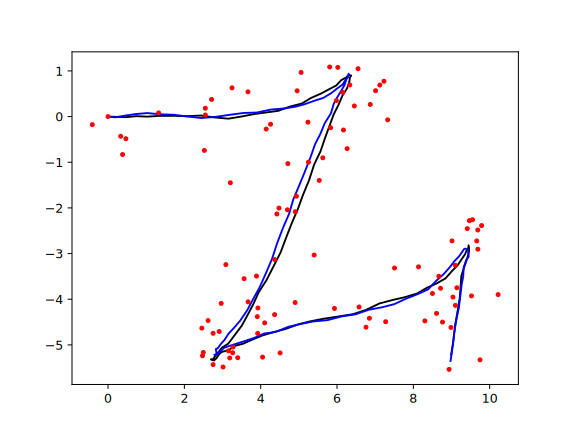
\includegraphics[width=0.85\textwidth,height=\textheight]{AdvFilteringFigures/particlefilter2.*}
\caption{The second Particle Filter applied to the motion of a
differential drive robot as above. This filter double samples the
physics, sorts the candidate particles and enforces a rank selection to
reduce to required population size. The simulation pose is given by the
blue line, the observation of the pose given by the red dots and the
pose estimate is given by the black line. 50 particles are used and the
average is the pose estimate.}
\end{figure}
